\chapter{Patrones de diseño}
Para la estructuración del proyecto en curso se contemplaron los siguientes patrones de diseño:
\leavevmode
\linebreak
\begin{itemize}
	\item{\textbf{Abstract Factory:} Abstract Factory es un patrón de diseño que provee una interfaz para la creación de familias de objetos o objetos dependientes relacionados entre sí sin especificar sus clases concretas.
	\begin{figure}[h!]
	\centering
		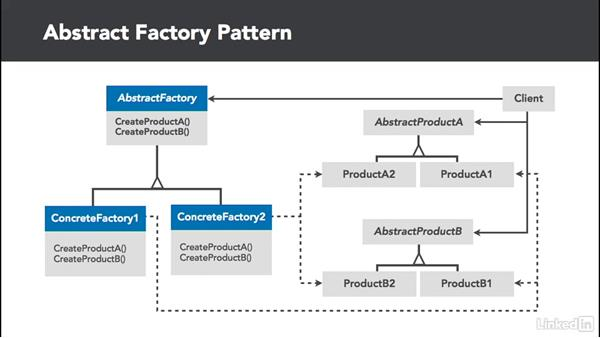
\includegraphics[scale=0.8]{diseno/patrones/imgs/abstractfactory}
		\caption{Patrón de diseño 'Abstract Factory'}
	\end{figure}
	Concretamente, se busca implementar este patrón de diseño para otorgar flexibilidad al momento de querer migrar todas operaciones y consultas de la base de datos a otro DBMS. Para este proyecto inicialmente se está trabajando con el DBMS PostgreSQL, pero si se quisiera migrar a otro tal como Oracle, MySQL u otro, este patrón otorga flexibilidad y facilidad para hacerlo. Para implementarlo, se parte de la base de que las operaciones sobre la base de datos se pueden ver como una familia de dos objetos: una conexión y un gestor. La conexión transportará todas las operaciones al DBMS que el gestor le solicite.
	\begin{figure}[h!]
	\centering
		\includegraphics[scale=0.7]{diseno/patrones/imgs/abstractfactoryDBMS}
		\caption{Patrón de diseño 'Abstract Factory' implementado dentro del proyecto}
	\end{figure}}
	\item{\textbf{Facade:} El patrón de diseño fachada provee una interfaz unificada para un conjunto de interfaces en un subsistema.
	\begin{figure}[h!]
	\centering
		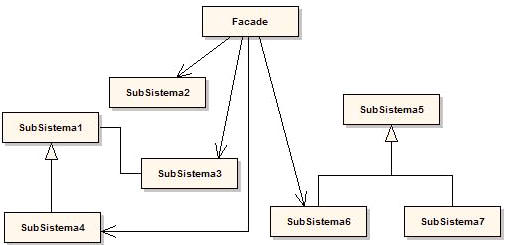
\includegraphics[scale=0.5]{diseno/patrones/imgs/facade}
		\caption{Patrón de diseño 'Facade'}
	\end{figure}	
	En el patrón de diseño 'Abstract Factory' que se planteó en el punto anterior, la interacción de la base de datos se da por medio de la clase 'DBFactory', que hace el papel de fábrica de los componentes que permiten dicha conexión; pero aquellos clientes que deseen interactuar y realizar operaciones con dicha conexión no deberían tener una relación con la clase 'DBFactory', de tal manera que se plantea el uso de una \textbf{Fachada} que establezca una interfaz que sirva de intermediaria entre ambas partes.
	\begin{figure}[h!]
	\centering
		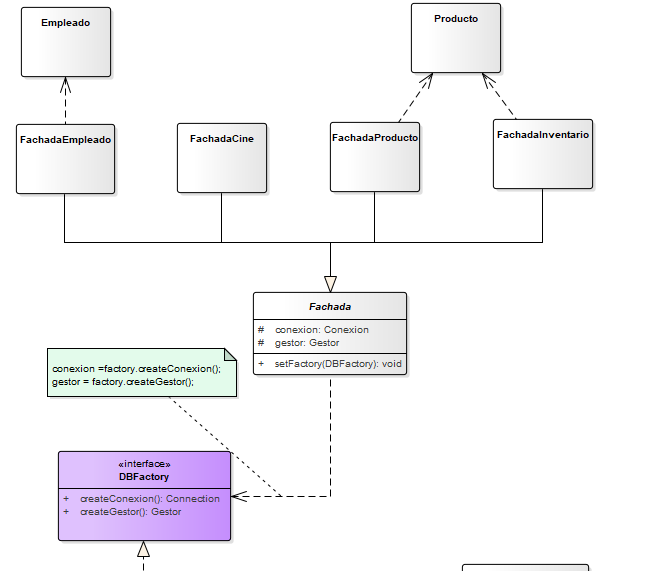
\includegraphics[scale=0.7]{diseno/patrones/imgs/facadeimplementado}
		\caption{Patrón de diseño 'Facade' implementado}
	\end{figure}
	}
	\item{\textbf{Singularidad (Patrón Prs):} El patrón de diseño de singularidad es un patrón -R el cuál es una mejora para la implementación relacionanda con el patrón singletón, con la ventaja de que mediante este patrón se pueden heredar todas las caraterísticas y ventajas que ofrece la clase padre.	
	\begin{figure}[h!]
	\centering
		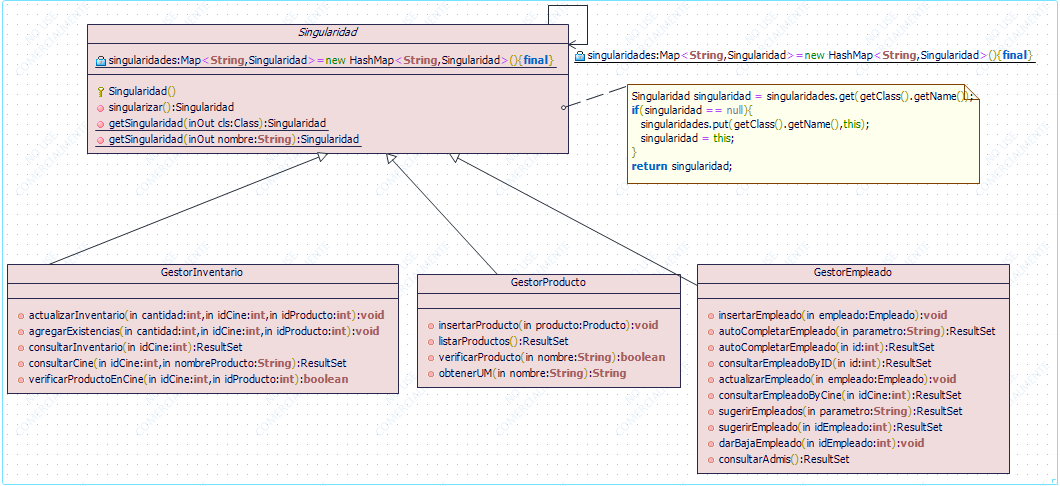
\includegraphics[scale=0.5]{diseno/patrones/imgs/singularidad}
		\caption{Patrón de diseño 'Singularidad' implementado}
	\end{figure}}
	
	 
\end{itemize}